\documentclass[12pt]{article}
\usepackage[left=1cm, right=1cm, top=2cm,bottom=1.5cm]{geometry} 

\usepackage[parfill]{parskip}
\usepackage[utf8]{inputenc}
\usepackage[T2A]{fontenc}
\usepackage[russian]{babel}
\usepackage{enumitem}
\usepackage[normalem]{ulem}
\usepackage{amsfonts, amsmath, amsthm, amssymb, mathtools}
\usepackage{tabularx}
\usepackage{hhline}

\usepackage{accents}
\usepackage{fancyhdr}
\pagestyle{fancy}
\renewcommand{\headrulewidth}{1.5pt}
\renewcommand{\footrulewidth}{1pt}

\usepackage{graphicx}
\usepackage[figurename=Рис.]{caption}
\usepackage{subcaption}
\usepackage{float}

%%Наименование папки откуда забирать изображения
\graphicspath{ {./images/} }

%%Изменение формата для ввода доказательства
\renewcommand{\proofname}{$\square$  \nopunct}
\renewcommand\qedsymbol{$\blacksquare$}

%%Изменение отступа на таблицах
\addto\captionsrussian{%
	\renewcommand{\proofname}{$\square$ \nopunct}%
}
%% Римские цифры
\newcommand{\RN}[1]{%
	\textup{\uppercase\expandafter{\romannumeral#1}}%
}

%% Для удобства записи
\newcommand{\MR}{\mathbb{R}}
\newcommand{\MQ}{\mathbb{Q}}
\newcommand{\MN}{\mathbb{N}}
\newcommand{\MI}{\mathrm{I}}
\newcommand{\MJ}{\mathrm{J}}
\newcommand{\MH}{\mathrm{H}}
\newcommand{\MT}{\mathrm{T}}
\newcommand{\MU}{\mathcal{U}}
\newcommand{\MV}{\mathcal{V}}
\newcommand{\VN}{\varnothing}
\newcommand{\VE}{\varepsilon}

\theoremstyle{definition}
\newtheorem{defn}{Опр:}
\newtheorem{rem}{Rm:}
\newtheorem{prop}{Утв.}
\newtheorem{exrc}{Упр.}
\newtheorem{lemma}{Лемма}
\newtheorem{theorem}{Теорема}
\newtheorem{corollary}{Следствие}

\newenvironment{cusdefn}[1]
{\renewcommand\thedefn{#1}\defn}
{\enddefn}

\DeclareRobustCommand{\divby}{%
	\mathrel{\text{\vbox{\baselineskip.65ex\lineskiplimit0pt\hbox{.}\hbox{.}\hbox{.}}}}%
}
%Короткий минус
\DeclareMathSymbol{\SMN}{\mathbin}{AMSa}{"39}
%Длинная шапка
\newcommand{\overbar}[1]{\mkern 1.5mu\overline{\mkern-1.5mu#1\mkern-1.5mu}\mkern 1.5mu}
%Функция знака
\DeclareMathOperator{\sgn}{sgn}

%Обозначение константы
\DeclareMathOperator{\const}{\text{const}}

%Интеграл в большом формате
\DeclareMathOperator{\dint}{\displaystyle\int}

\newcommand{\smallerrel}[1]{\mathrel{\mathpalette\smallerrelaux{#1}}}
\newcommand{\smallerrelaux}[2]{\raisebox{.1ex}{\scalebox{.75}{$#1#2$}}}

\newcommand{\smallin}{\smallerrel{\in}}
\newcommand{\smallnotin}{\smallerrel{\notin}}

\newcommand*{\medcap}{\mathbin{\scalebox{1.25}{\ensuremath{\cap}}}}%
\newcommand*{\medcup}{\mathbin{\scalebox{1.25}{\ensuremath{\cup}}}}%

\makeatletter
\newcommand{\vast}{\bBigg@{3.5}}
\newcommand{\Vast}{\bBigg@{5}}
\makeatother

%Скалярное произведение
\DeclarePairedDelimiterX{\inner}[2]{\langle}{\rangle}{#1, #2}

%Подпись символов снизу
\newcommand{\ubar}[1]{\underaccent{\bar}{#1}}

\begin{document}
\lhead{Математический анализ - \RN{2}}
\chead{Шапошников С.В.}
\rhead{Лекция - 14}
	
\section*{Правила дифференцировани}
В прошлый раз рассмотрели правила дифференцирования в общем случае. 

\begin{theorem} \textbf{Дифференцирование сложной функции}: 
	Пусть $X, Y, Z$ - нормированные пространства, функция $f \colon X \to Y$ - дифференцируема в точке $a \in X$, функция $g\colon Y \to Z$ - дифференцируема в точке $f(a)$. Тогда $g(f(x))$ - дифференцируема в точке $a$ и верно следующее:
	$$
		dg \circ f = dg \circ df
	$$
\end{theorem}

Сложность заключается в переходе на конкретные примеры. 

\section*{Частные случаи дифференцируемости сложных функций}
\subsection*{$(\RN{1})$ Функции из $\MR^n$ в $\MR^m$, из $\MR^m$ в $\MR^k$}
Пусть $f \colon \MR_x^n \to \MR_y^m, \, g \colon \MR_y^m \to \MR^k$, тогда:
$$
	df(h) = \begin{pmatrix}
		\tfrac{\partial f_1}{\partial x_1} &  \dotsc & \tfrac{\partial f_1}{\partial x_n} \\
		\vdots & \ddots & \vdots \\
		\tfrac{\partial f_m}{\partial x_1} & \dotsc & \tfrac{\partial f_m}{\partial x_n} 			
	\end{pmatrix}{\cdot}
	\begin{pmatrix}
		h_1\\
		\vdots\\
		h_n
	\end{pmatrix} = J_f{\cdot} h, \, 
	dg(v) = \begin{pmatrix}
		\tfrac{\partial g_1}{\partial y_1} &  \dotsc & \tfrac{\partial g_1}{\partial y_m} \\
		\vdots & \ddots & \vdots \\
		\tfrac{\partial g_k}{\partial y_1} & \dotsc & \tfrac{\partial g_k}{\partial y_m} 			
	\end{pmatrix}{\cdot}
	\begin{pmatrix}
		v_1\\
		\vdots\\
		v_m
	\end{pmatrix} = J_g{\cdot}v
$$
В этом случае, композиция запишется следующим образом:
$$
	f \colon x =\begin{pmatrix}
		x_1\\
		\vdots\\
		x_n
	\end{pmatrix} \to
	\begin{pmatrix}
		f_1(x)\\
		\vdots\\
		f_m(x)
	\end{pmatrix}, \, 
	g \colon y = \begin{pmatrix}
		y_1\\
		\vdots\\
		y_m
	\end{pmatrix} \to
	\begin{pmatrix}
		g_1(y)\\
		\vdots\\
		g_k(y)
	\end{pmatrix} \Rightarrow 
$$
$$
	\Rightarrow	g\big(f(x)\big) = 
	\begin{pmatrix}
		g_1\big(f_1(x_1,\dotsc, x_n),  \dotsc, f_m(x_1, \dotsc, x_n) \big)\\
		\vdots\\
		g_k\big(f_1(x_1,\dotsc, x_n),  \dotsc, f_m(x_1, \dotsc, x_n) \big)
	\end{pmatrix}
$$
Как выглядит дифференциал в таком случае? С одной стороны, он будет иметь следующий вид:
$$
	d(g\circ f)(h) = dg(f)(h) = \begin{pmatrix}
		\tfrac{\partial g_1(f(x))}{\partial x_1} &  \dotsc & \tfrac{\partial g_1(f(x))}{\partial x_n} \\
		\vdots & \ddots & \vdots \\
		\tfrac{\partial g_k(f(x))}{\partial x_1} & \dotsc & \tfrac{\partial g_k(f(x))}{\partial x_n} 			
	\end{pmatrix}{\cdot}
	\begin{pmatrix}
		h_1\\
		\vdots\\
		h_n
	\end{pmatrix} = J_{g(f)}{\cdot}h
$$
Получили матрицу Якоби функции $g(f)$. C другой стороны, это должно быть композицей двух дифференциалов $df(h)$ и $dg(v)$, распишем их по определению:
$$
	\big(dg \circ df\big) (h) = dg\big(df(h)\big) = dg \big(J_f{\cdot}h \big) = J_g{\cdot}(J_f{\cdot}h)
$$
Распишем дифференцирование сложной функции подробнее:
$$
	d(g\circ f)(h) =  J_{g(f)}{\cdot}h = J_g{\cdot}(J_f{\cdot}h) = \big(dg \circ df\big) (h)
$$
$$	
	\begin{pmatrix}
		\tfrac{\partial g_1(f(x))}{\partial x_1} &  \dotsc & \tfrac{\partial g_1(f(x))}{\partial x_n} \\
		\vdots & \ddots & \vdots \\
		\tfrac{\partial g_k(f(x))}{\partial x_1} & \dotsc & \tfrac{\partial g_k(f(x))}{\partial x_n} 			
	\end{pmatrix}{\cdot}
	\begin{pmatrix}
		h_1\\
		\vdots\\
		h_n
	\end{pmatrix} = 
	\begin{pmatrix}
		\tfrac{\partial g_1}{\partial y_1} &  \dotsc & \tfrac{\partial g_1}{\partial y_m} \\
		\vdots & \ddots & \vdots \\
		\tfrac{\partial g_k}{\partial y_1} & \dotsc & \tfrac{\partial g_k}{\partial 		y_m} 			
	\end{pmatrix}{\cdot}
	\begin{pmatrix}
		\tfrac{\partial f_1}{\partial x_1} &  \dotsc & \tfrac{\partial f_1}{\partial x_n} \\
		\vdots & \ddots & \vdots \\
		\tfrac{\partial f_m}{\partial x_1} & \dotsc & \tfrac{\partial f_m}{\partial x_n} 			
	\end{pmatrix}{\cdot}
	\begin{pmatrix}
		h_1\\
		\vdots\\
		h_n
	\end{pmatrix} 
$$
Как устроены элементы матрицы Якоби $J_{g(f)}$, рассмотрим подробнее:
$$
	\dfrac{\partial g_l}{\partial x_s} = \dfrac{\partial g_l}{\partial y_1}{\cdot}\dfrac{\partial f_l}{\partial x_s} + \dotsc + \dfrac{\partial g_l}{\partial y_m}{\cdot}\dfrac{\partial f_m}{\partial x_s}, \, l = \overline{1,k}, \, s = \overline{1,n}
$$
\newpage
\subsection*{$(\RN{2})$ Функции из $\MR$ в $\MR^2$, из $\MR^2$ в $\MR$}

Пусть $g \colon \MR^2 \to \MR$  - дифференцируема в каждой точке. Рассматрим отображение $\MR \to \MR^2$, которое устроено так: $t \mapsto (x_1(t), x_2(t))$, где $x_i$ - дифференцируемые функции. На основе этого отображения построим новую функцию: 
$$
	t \mapsto (x_1(t), x_2(t)) \mapsto g(x_1(t),x_2(t))
$$ 
Отображение рисует некоторую кривую $(x_1(t),x_2(t))$, а затем мы смотрим, как функция $g$ меняется вдоль этой кривой. Таким образом, нам нужно посмотреть как устроена функция: $f(t) = g(x_1(t),x_2(t))$.
\begin{figure}[H]
	\centering
	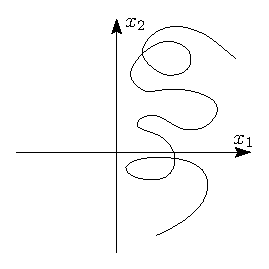
\includegraphics[width=0.25\textwidth]{14_1.eps}
	\caption{Отображение $t \mapsto (x_1(t),x_2(t))$.}
	\label{14_1}
\end{figure}
Первое, что обычно хотят понять, как устроена производная такой функции (заметим, фукнции одной переменной). Рассмотрим дифференциал $f$:
$$
	df(v) = dg 
	\renewcommand\arraystretch{1.2}
	\begin{pmatrix}
		\begin{pmatrix}
			\tfrac{\partial x_1}{\partial t}\\
			\tfrac{\partial x_2}{\partial t}
		\end{pmatrix} \! v
	\end{pmatrix}
	= dg 
	\begin{pmatrix}
		\begin{pmatrix}
			\dot{x}_1\\
			\dot{x}_2
		\end{pmatrix} \! v
	\end{pmatrix} = 
	\begin{pmatrix}
		\dfrac{\partial g}{\partial x_1} & \dfrac{\partial g}{\partial x_2}
	\end{pmatrix}{\cdot}
	\begin{pmatrix}
		\dot{x}_1\\
		\dot{x}_2
	\end{pmatrix} \! v
$$
Перепишем это выражение в производных (опуская домножение на вектор $v$):
$$
	\dfrac{df}{dt} = \dfrac{\partial g}{\partial x_1}{\cdot}\dot{x}_1 + \dfrac{\partial g}{\partial x_2}{\cdot}\dot{x}_2
$$
Докажем этот частный случай еще раз, для лучшего понимания. 
\begin{proof}
	Рассмотрим производную функции $f$ по переменной $t$:
	$$
		\dfrac{df}{dt}\bigg|_{t = t_0} = \dfrac{d}{dt}g\big(x_1(t),x_2(t)\big)\bigg|_{t = t_0} = \lim\limits_{t \to t_0}\dfrac{g\big(x_1(t),x_2(t)\big) - g\big(x_1(t_0),x_2(t_0)\big)}{t - t_0} =
	$$
	$$
	 	= \lim\limits_{t \to t_0} \vast(\dfrac{\tfrac{\partial g}{\partial x_1} \big(x_1(t_0), x_2(t_0)\big)\big(x_1(t) - x_1(t_0)\big) + \tfrac{\partial g}{\partial x_2} \big(x_1(t_0), x_2(t_0)\big)\big(x_2(t) - x_2(t_0)\big)}{t - t_0} + 
	$$
	$$
	 	+ \dfrac{
	 		\alpha\big(x_1(t) - x_1(t_0), x_2(t) - x_2(t_0) \big){\cdot}
	 		\sqrt{
	 			\big(x_1(t) - x_1(t_0)\big)^2 + \big(x_2(t) - x_2(t_0)\big)^2 
			} 
	 	}{t - t_0}\vast) = 
	$$
	Переопределим $\alpha(h)$ таким образом, что $\alpha(0) = 0$ и внесем $t - t_0$ под каждый из членов в отдельности:
	$$
		= \lim\limits_{t \to t_0} \Bigg(\dfrac{\partial g}{\partial x_1}{\cdot}\dfrac{x_1(t) - x_1(t_0)}{t - t_0} + \dfrac{\partial g}{\partial x_2}{\cdot}\dfrac{x_2(t) - x_2(t_0)}{t - t_0} + 
	$$
	$$
		+ \alpha\big(x_1(t) - x_1(t_0), x_2(t) - x_2(t_0) \big){\cdot}\dfrac{1}{\sgn{(t-t_0)}}{\cdot} \sqrt{\bigg(\dfrac{x_1(t) - x_1(t_0)}{t - t_0}\bigg)^2 + \bigg(\dfrac{x_2(t) - x_2(t_0)}{t - t_0}\bigg)^2} \Bigg) = 
	$$
	$$
		= \dfrac{\partial g}{\partial x_1}{\cdot}\dot{x}_1(t_0) + \dfrac{\partial g}{\partial x_2}{\cdot}\dot{x}_2(t_0) + 0 = \dfrac{\partial g}{\partial x_1}{\cdot}\dot{x}_1(t_0) + \dfrac{\partial g}{\partial x_2}{\cdot}\dot{x}_2(t_0)
	$$
\end{proof}

\section*{Частные случаи дифференцируемости обратной функции}
Вспомним, о чем говорит теорема о дифференцируемости обратной функции. Если выполнены условия теоремы, то мы знаем, что дифференциал обратной функции $df^{-1}$ есть обратное отображение к дифференциалу функции $(df)^{-1}$.
\begin{theorem} \textbf{О дифференцируемости обратной функции}: 
	Пусть $X, Y$ - нормированные пространства, множества $\MU \subset X, \, \MV \subset Y$ - открытые. Если функция $f \colon \MU \to \MV$ - гомеоморфизм (биекция, отображение и обратное к нему - непрерывны), $f$ - дифференцируема в точке $a \in \MU$ и $df \colon X \to Y$ имеет  обратный оператор $(df)^{-1} \colon Y \to X$ - непрерывный линейный оператор. Тогда функция $f^{-1}\colon \MV \to \MU$ является дифференцируемой в точке $f(a)$ и $df^{-1} = (df)^{-1}$.
\end{theorem}

\subsection*{Функции из $\MR^n$ в $\MR^n$}

Рассмотрим $f \colon \MR^n \to \MR^n$. Пусть оно удовлетворяет условиям теоремы о дифференцируемости обратной функции (везде или в точке). Тогда, если $df(v) = J_f{\cdot}v$, то:
$$
	df^{-1}(v) = J_{f^{-1}}{\cdot}v =  J_f^{-1}{\cdot}v = (df)^{-1}(v)
$$	
Как найти обратную к матрице Якоби? Надо найти матрицу Якоби обратного отображения:
$$
	J_{f^{-1}} = J_f^{-1}
$$
По-другому, если отображение $f\colon y = y(x)$, то получить матрицу Якоби отображения $x = x(y)$ можно следующим образом:
$$
	J_f = \bigg(\dfrac{\partial y_i}{\partial x_j}\bigg)_{i,j} \Rightarrow  J_{f^{-1}} = \bigg(\dfrac{\partial x_j}{\partial y_i}\bigg)_{i,j} =  \bigg(\dfrac{\partial y_i}{\partial x_j}\bigg)^{-1}_{i,j} = (J_f)^{-1}
$$

\subsection*{Типичная задача} 
Заданы уравнения $x = \varphi(u,v), \, y = \psi(u,v)$. То есть:
$$
	(x,y) = f(u,v) = \big(\varphi(u,v), \psi(u,v)\big)
$$

Предполагается, что это хорошая замена и можно выразить $u, \, v$ через $x, \, y$ и она удовлетворяет всем свойствам теоремы о дифференцируемости обратной функции. Нужно найти все частные производные $\dfrac{\partial u}{\partial x}, \, \dfrac{\partial v}{\partial x}, \, \dfrac{\partial u}{\partial y}, \, \dfrac{\partial v}{\partial y}$ этих уравнений. Как решать? Продифференцируем по $x$ и получим:
$$
	1 = \dfrac{\partial \varphi}{\partial u}{\cdot}\dfrac{\partial u}{\partial x} + \dfrac{\partial \varphi}{\partial v}{\cdot}\dfrac{\partial v}{\partial x}, \,
	0 = \dfrac{\partial \psi}{\partial u}{\cdot}\dfrac{\partial u}{\partial x} + \dfrac{\partial \psi}{\partial v}{\cdot}\dfrac{\partial v}{\partial x}
$$
Отсюда выражаются нужные частные производные и затем то же самое делается для $y$. 
$$
	0 = \dfrac{\partial \varphi}{\partial u}{\cdot}\dfrac{\partial u}{\partial y} + \dfrac{\partial \varphi}{\partial v}{\cdot}\dfrac{\partial v}{\partial y}, \,
	1 = \dfrac{\partial \psi}{\partial u}{\cdot}\dfrac{\partial u}{\partial y} + \dfrac{\partial \psi}{\partial v}{\cdot}\dfrac{\partial v}{\partial y}
$$
Но здесь на самом деле записано, что если взять матрицу Якоби отображения $f\colon (u,v) \to (x,y)$ и умножить на матрицу Якоби обратного отображения $f^{-1}\colon (x,y) \to (u,v)$, то получим единичную матрицу:
$$
	\renewcommand\arraystretch{1.2}
	\begin{pmatrix}
		1 & 0 \\
		0 & 1 
	\end{pmatrix} = 
	\begin{pmatrix}
		\tfrac{\partial \varphi}{\partial u} & \tfrac{\partial \varphi}{\partial v}\\
		\tfrac{\partial \psi}{\partial u} & \tfrac{\partial \psi}{\partial v}
	\end{pmatrix}{\cdot}
	\begin{pmatrix}
		\tfrac{\partial u}{\partial x} & \tfrac{\partial u}{\partial x}\\
		\tfrac{\partial v}{\partial x} & \tfrac{\partial v}{\partial y}
	\end{pmatrix} =J_f{\cdot}J_{f^{-1}}
$$
Это ровно то правило, которое утверждает, что матрица Якоби обратного отображения это обратная матрица Якоби исходного отображения.

\begin{rem}
	Дифференцирование обратной функции может быть полезно еще с одной стороны.	Мы знаем, что если $f$ дифференцируема, то при $x \approx a$ мы имеем локально аффинное отображение (т.е. сдвиг плюс линейное отображение):
	$$
		f(x) \approx f(a) + J_f{\cdot}(x-a)
	$$
	Теперь хотим найти обратное отображение к $y = f(x)$, то есть буквально выразить $x$ через $y \Rightarrow$ как найти $f^{-1}$? Нужно решить уравнение $y = f(x)$ и найти чему равен $x$, что в явном виде во многих случаях почти невозможно. Используя дифференцирование обратной функции можем использовать приближение выше, тогда при $y \approx f(a)$ получим:
	$$
		f^{-1}(y) \approx a + \big(f^\prime(a)\big)^{-1}{\cdot}\big(y - f(a)\big) = a + 	J_f^{-1}{\cdot}\big(y - f(a)\big)
	$$
	И в этом случае система превращается в линейную, которая уже хорошо решается.
\end{rem}

\begin{rem}
	При этом хочется отметить, что теорема о дифференцируемости обратной функции достаточно сложна в использовании из-за множества условий. Кроме того, она не утверждает, что обратная функция существует, это занесено в условие вместе с тем, что это непрерывная функция.
\end{rem}

\newpage
\section*{Теорема об обратной функции}
\subsection*{Одномерный случай: $\MR$}
В первом семестре была теорема, в которой утверждалось существование обратной функции:
\begin{theorem}\textbf{(Об обратной функции в $\MR$)}
	Пусть $\MI \neq \VN$ промежуток и $f \colon \MI \to \MR$ - непрерывная, строго монотонная функция. Тогда 
	\begin{enumerate}[label={\arabic*)}]
		\item $f(\MI) = \MJ = \{\, y \colon \exists \, x \in \MI, f(x) = y \,\}$ - непустой промежуток;
		\item $f\colon \MI \to \MJ$ - биекция;
		\item $f^{-1} \colon \MJ \to \MI$ - строго монотонна и непрерывна;
	\end{enumerate}
\end{theorem}

\begin{corollary}
	Пусть $f$ - непрерывно дифференцируема в окрестности точки $a$ и $f^\prime(a) \neq 0$. Тогда существует интервалы $\MU(a)$ и $\MV\big(f(a)\big)$ такие, что $f\colon \MU \to \MV$ - гомеоморфизм и $f^{-1}$ непрерывно дифференцируема на $\MV$.
\end{corollary}
\begin{defn}
	Если функция $f\colon \MU \to \MV$ - биекция, такая что $f, f^{-1}$ - непрерывно дифференцируемы, то говорят, что задан \uwave{диффеоморфизм}.
\end{defn}

\begin{rem}
	Таким образом, $f$ локально это диффеоморфизм окрестностей точек $a$ и $f(a)$, когда $f^\prime(a) \neq 0$.
\end{rem}

\begin{proof}
	Докажем следствие, используя строгую монотонность. \hfill\\
	Поскольку $f$ - непрерывно дифференцируема в окрестности точки $a$ (то есть $f^\prime(x)$ - непрерывно в окрестности точки $a$) и $f^\prime(a) \neq 0$, пусть $f^\prime(a) > 0$, тогда $\exists \, (a-\delta, a + \delta) = \MI \colon f^\prime(x) > 0$. Тогда на этом интервале $f$ строго возрастает, то есть $f$ строго монотонна на интервале $\MI \Rightarrow \MJ = f(\MI)$ - интервал, $f\colon \MI \to \MJ$ - биекция и обратная функция $f^{-1} \colon \MJ \to \MI$ - непрерывна и строго монотонна. 
	
	Мы получили гомеоморфизм и $\forall x \in \MI, \, f^\prime(x) > 0$, тогда обратное отображение в этой точке дифференцируемо и 
	$(f^{-1})^\prime = \tfrac{1}{f^\prime}$ (по теореме о дифференцируемости обратной функции). Поскольку $\tfrac{1}{f^\prime}$ - непрерывная функция, то мы получили не только дифференцируемость обратной функции, но еще и её непрерывную дифференцируемость.
\end{proof}

В общем случае такого утверждения нет, поскольку нет простого свойства монотонности, нет отношения порядка на плоскости. Но хотелось бы какое-то простое условие, гарантирующее гомеоморфизм (хотя бы локально). 

\subsection*{Теорема Банаха для общего случая: $\MR^n$}
Пусть $f\colon \MR^n \to \MR^n$ и мы хотим найти обратную функцию/понять, что она существует? У нас есть функция $y = f(x)$, а хотим найти $f^{-1} \colon y \to x$ или по-другому - решить уравнение $y = f(x)$, как уравнение на $x$ относительно $y$. Таким образом, построить $f^{-1} \Leftrightarrow$ решить уравнение $y = f(x)$ относительно $x$.
$$
	\left\{\begin{array}{lcl}
		y_1  &=& f_1(x_1,\dotsc, x_n)\\
		   &\vdots& \\
		y_n  &=& f_n(x_1,\dotsc, x_n)
	\end{array}\right.
$$
Решать системы уравнений мы умеем, когда они линейные, но эта система - нелинейная и в лоб решить её не получится.

\textbf{\uline{Идея}}: Свести решение уравнения к поиску неподвижной точки, то есть свести решение задачи к уравнению $x = F(x)$. Способ сведения будет следующим:
$$
	y = f(x) \Leftrightarrow x = x + Q(y - f(x))
$$
где $Q$ - невырожденная матрица. Почему это лучше? Потому что, как искать неподвижные точки мы знаем (чаще всего это задачи вида: $x_{n+1} = F(x_n)$).
\begin{theorem}
	\textbf{(Банаха)} Пусть $(X,\rho)$ - полное метрическое пространство и $F \colon X \to X$ - сжимающее отображение с коэффициентом сжатия $0 < q < 1$, то есть:
	$$
		\rho(F(x_1),F(x_2)) \leq q{\cdot}\rho(x_1,x_2), \, \forall x_1, x_2
	$$
	Тогда существует единственная точка $x_0 \in X \colon F(x_0) = x_0$, где $x_0$ называется \uwave{неподвижной точкой} $F$. 
\end{theorem}
\begin{rem}
	Данное утверждение хорошо тем, что оно четко выделяет что нужно проверять, чтобы доказать, существование неподвижной точки. Более того, поскольку помимо решения уравнения нас интересует построение обратной функции (т.е. чтобы каждому $y$ соответствовал единственный $x$), эта теорема дает не только существование, но и единственность такой точки.
\end{rem}
\begin{proof}\hfill\\
	\uwave{Единственность}: Пусть $x_0$ и $y_0$ - неподвижные точки, тогда:
	$$
		\rho(x_0,y_0) = \rho\big(F(x_0),F(y_0)\big) \leq q{\cdot}\rho(x_0,y_0), \, 0 < q < 1 \Rightarrow \underbrace{(1-q)}_{> 0}{\cdot}\rho(x_0,y_0) \leq 0 \Rightarrow \rho(x_0,y_0) = 0 \Rightarrow x_0 = y_0
	$$
	Таким образом, такая точка только одна.
	
	\uwave{Существование}: Возьмем последовательность $x_{n+1} = F(x_n)$, где $x_1$ - произвольная точка $X$, тогда получим последовательность вида:
	$$
		x_1, F(x_1), F\big(F(x_1)\big), \dotsc 
	$$
	Докажем, что $x_n$ сходится через критерий Коши, то есть покажем, что $x_n$ - фундаментальна. Рассмотрим сначала ``неправильную'' оценку (поскольку для доказательства необходимо расстояние между любыми двумя членами):
	$$
		\rho(x_{n+1},x_n) = \rho\big(F(x_n), F(x_{n-1})\big) \leq q{\cdot}\rho(x_n, x_{n-1}) \leq q^2 {\cdot}\rho(x_{n-1}, x_{n-2}) \leq \dotsc \leq q^{n-1} {\cdot}\rho(x_2,x_1)
	$$
	Оценим расстояние между любыми двумя членами последовательности $n > m$, используя неравенство треугольника:
	$$
		\rho(x_n,x_m) \leq \rho(x_n, x_{n-1}) + \rho(x_{n-1},x_{n-2}) + \dotsc + \rho(x_{m+1},x_m)
	$$
	Тогда, используя ``неправильную'' оценку мы получим следующее:
	$$
		\rho(x_n,x_m) \leq q^{n-2}{\cdot}\rho(x_2,x_1) + \dotsc + q^m{\cdot}\rho(x_2,x_1) +  q^{m-1}{\cdot}\rho(x_2,x_1)  \leq  
	$$
	$$
		\leq q^{m-1}{\cdot}\rho(x_2,x_1) + q^m{\cdot}\rho(x_2,x_1) + \dotsc + q^{n-2}{\cdot}\rho(x_2,x_1) + q^{n-1}{\cdot}\rho(x_2,x_1) + \dotsc = \dfrac{\rho(x_2,x_1){\cdot}q^{m-1}}{1- q}
	$$
	Поскольку $0 < q < 1$, то для произвольного $\VE > 0$ найдется такой достаточно большой $N$, что будет верно следующее неравенство:
	$$	
		\forall n, m > N, \, \rho(x_n, x_m) \leq \dfrac{\rho(x_2,x_1){\cdot}q^{N-1}}{1- q} < \VE
	$$
	Следовательно $x_n$ - фундаментальна и $\exists \, \lim\limits_{n\to \infty}x_n = x_0$.
	\begin{rem}
		На самом деле, мы доказали немного больше, чем существование предела, поскольку мы можем сказать, как быстро сходится к этому пределу последовательность. Если $n \to \infty$, то $\rho(x_0, x_m) \leq C{\cdot}q^m$.
	\end{rem}
	Поскольку $F$ - непрерывное отображение $\Rightarrow \lim\limits_{n \to \infty}F(x_n) = F(x_0)$, тогда:
	$$
		F(x_0) = \lim\limits_{n\to \infty} F(x_n) = \lim\limits_{n\to \infty} x_{n+1} = x_0
	$$
	и таким образом $F(x_0) = x_0$.
\end{proof}
На самом деле, этого утверждения нам мало, поскольку мы хотим построить не просто обратную функцию, а обратную имеющие некие свойства, например, непрерывность. Нам необходимо понимать, как меняется $x$, когда меняется $y$. Правда ли, что если отображения отличаются мало, то и неподвижные точки отличаются мало?
\begin{rem}
	Пусть $(X,\rho)$ - полное метрическое пространство, $F, G\colon X \to X$ - сжимающиеся отображения с коэффициентом сжатия $q$ (если разные, то возьмем самый большой). Пусть $x_f$ и $x_g$ - это их неподвижные точки. Хотим оценить расстояние между этими двумя неподвижными точками. Применяя неравенство треугольника получим:
	$$
		\rho(x_f,x_g) = \rho\big(F(x_f),G(x_g) \big) \leq \rho\big(F(x_f),F(x_g)\big) + \rho\big(F(x_g),G(x_g) \big)
	$$
	Поскольку $F$ - сжимающее отображение,то получим следующее:
	$$
		\rho\big(F(x_f),F(x_g)\big) + \rho\big(F(x_g),G(x_g) \big) \leq q{\cdot}\rho(x_f,x_g) + \rho\big(F(x_g),G(x_g)\big)
	$$
	Перенесем $\rho(x_f,x_g)$ в левую часть и разделим на коэффициент $(1-q)$, получим оценку:
	$$
		\rho(x_f,x_g) \leq \dfrac{1}{1-q}{\cdot}\rho\big(F(x_g),G(x_g) \big)
	$$
	Таким образом, если отображения $F$ и $G$ мало отличаются во всех точках, то и точки $x_f, x_g$ будут отличаться мало.
\end{rem}

\end{document}